\definecolor{c6c8ebf}{RGB}{108,142,191}
\definecolor{cdae8fc}{RGB}{218,232,252}
\definecolor{c82b366}{RGB}{130,179,102}
\definecolor{cd5e8d4}{RGB}{213,232,212}
\definecolor{c666666}{RGB}{102,102,102}
\definecolor{whitesmoke}{RGB}{245,245,245}
\definecolor{c333333}{RGB}{51,51,51}


\def \globalscale {0.900000}
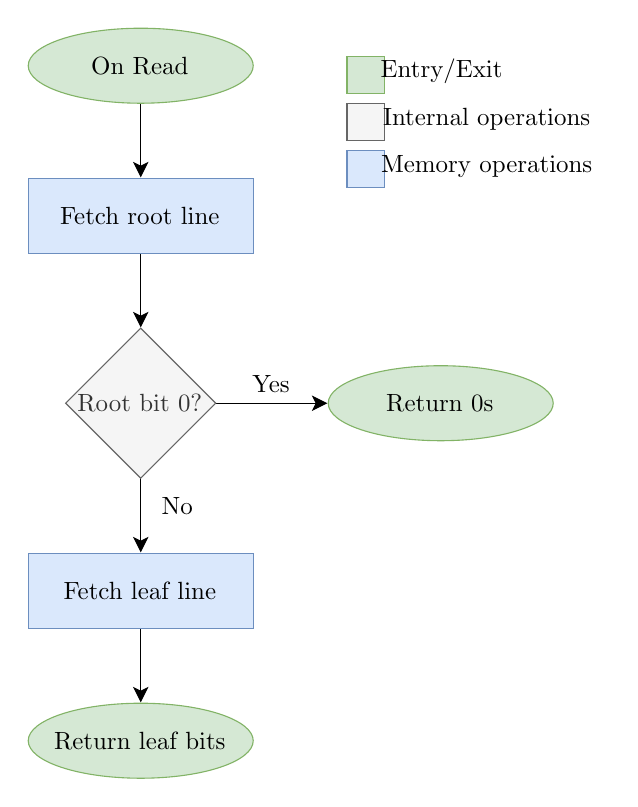
\begin{tikzpicture}[y=1cm, x=1cm, yscale=\globalscale,xscale=\globalscale, every node/.append style={scale=\globalscale}, inner sep=0pt, outer sep=0pt]
  \path[draw=black,miter limit=10.0] (1.5875, 7.4348) -- (1.5875, 6.545);



  \path[draw=black,fill=black,miter limit=10.0] (1.5875, 6.4061) -- (1.4949, 6.5913) -- (1.5875, 6.545) -- (1.6801, 6.5913) -- cycle;



  \path[draw=c6c8ebf,fill=cdae8fc] (0.0, 8.4931) rectangle (3.175, 7.4348);



  \begin{scope}[fill=black,anchor=south]
    \node[text=black,anchor=south] (text2751) at (1.5743, 7.8449){Fetch root line};



  \end{scope}
  \path[draw=black,miter limit=10.0] (1.5875, 9.5515) -- (1.5875, 8.6617);



  \path[draw=black,fill=black,miter limit=10.0] (1.5875, 8.5228) -- (1.4949, 8.708) -- (1.5875, 8.6617) -- (1.6801, 8.708) -- cycle;



  \path[draw=c82b366,fill=cd5e8d4] (1.5875, 10.0806) ellipse (1.5875cm and 0.5292cm);



  \begin{scope}[fill=black,anchor=south]
    \node[text=black,anchor=south] (text9098) at (1.5743, 9.9616){On Read};



  \end{scope}
  \path[draw=black,miter limit=10.0] (2.6458, 5.3181) -- (4.0648, 5.3181);



  \path[draw=black,fill=black,miter limit=10.0] (4.2037, 5.3181) -- (4.0185, 5.2255) -- (4.0648, 5.3181) -- (4.0185, 5.4107) -- cycle;



  \path[draw=black,miter limit=10.0] (1.5875, 4.2598) -- (1.5875, 3.37);



  \path[draw=black,fill=black,miter limit=10.0] (1.5875, 3.2311) -- (1.4949, 3.4163) -- (1.5875, 3.37) -- (1.6801, 3.4163) -- cycle;



  \path[draw=c666666,fill=whitesmoke,miter limit=10.0] (1.5875, 6.3765) -- (2.6458, 5.3181) -- (1.5875, 4.2598) -- (0.5292, 5.3181) -- cycle;



  \begin{scope}[fill=c333333,anchor=south]
    \node[text=c333333,anchor=south] (text9223) at (1.5743, 5.1991){Root bit 0?};



  \end{scope}
  \path[draw=c82b366,fill=cd5e8d4] (5.8208, 5.3181) ellipse (1.5875cm and 0.5292cm);



  \begin{scope}[fill=black,anchor=south]
    \node[text=black,anchor=south] (text4055) at (5.8076, 5.1991){Return 0s};



  \end{scope}
  \path (2.6458, 5.9796) rectangle (4.2333, 5.1858);



  \begin{scope}[fill=black,anchor=south]
    \node[text=black,anchor=south] (text9546) at (3.4264, 5.4636){Yes};



  \end{scope}
  \path[draw=black,miter limit=10.0] (1.5875, 2.1431) -- (1.5875, 1.614) -- (1.5875, 1.2533);



  \path[draw=black,fill=black,miter limit=10.0] (1.5875, 1.1144) -- (1.4949, 1.2996) -- (1.5875, 1.2533) -- (1.6801, 1.2996) -- cycle;



  \path[draw=c6c8ebf,fill=cdae8fc] (0.0, 3.2015) rectangle (3.175, 2.1431);



  \begin{scope}[fill=black,anchor=south]
    \node[text=black,anchor=south] (text3383) at (1.5743, 2.5532){Fetch leaf line};



  \end{scope}
  \path (1.3229, 4.2598) rectangle (2.9104, 3.466);



  \begin{scope}[fill=black,anchor=south]
    \node[text=black,anchor=south] (text6126) at (2.1034, 3.7439){No};



  \end{scope}
  \path[draw=c82b366,fill=cd5e8d4] (1.5875, 0.5556) ellipse (1.5875cm and 0.5292cm);



  \begin{scope}[fill=black,anchor=south]
    \node[text=black,anchor=south] (text4320) at (1.5743, 0.4366){Return leaf bits};



  \end{scope}
  \path[draw=c82b366,fill=cd5e8d4] (4.4979, 10.2129) rectangle (5.0271, 9.6838);



  \path (4.9213, 10.3452) rectangle (6.7733, 9.5515);



  \begin{scope}[fill=black,anchor=south]
    \node[text=black,anchor=south] (text906) at (5.8341, 9.8293){Entry/Exit};



  \end{scope}
  \path[draw=c666666,fill=whitesmoke] (4.4979, 9.5515) rectangle (5.0271, 9.0223);



  \path (4.8948, 9.6838) rectangle (8.0698, 8.89);



  \begin{scope}[fill=black,anchor=south]
    \node[text=black,anchor=south] (text5276) at (6.4691, 9.1678){Internal operations};



  \end{scope}
  \path[draw=c6c8ebf,fill=cdae8fc] (4.4979, 8.89) rectangle (5.0271, 8.3608);



  \path (4.7625, 9.0223) rectangle (8.2021, 8.2285);



  \begin{scope}[fill=black,anchor=south]
    \node[text=black,anchor=south] (text6516) at (6.4691, 8.5064){Memory operations};



  \end{scope}

\end{tikzpicture}
